% !TEX root = main.tex

\section{Proofs}
In this appendix, we present the proofs of different theoretical results presented in the paper.
\subsection{Proof of Proposition \ref{prop:reward_attack}}\label{app:proof_prop_rewd_attack}

\begin{prop*}
	For any $\delta\in(0, 1/K]$, when using Contextual ACE algorithm (Alg. ~\ref{alg:attacker_rewards}) with perturbed rewards $\tilde{r}^{1}$, with probability at least $1-K\delta$, algorithm $\mathfrak{A}$ pulls \changelm{an arm in $A^{\dagger}$} for $T - o(T)$ time steps and the total cost of attacks is $o(T)$.
\end{prop*}

\begin{proof}
	Let us consider the contextual bandit problem $\mathcal{A}_{1}$, with $K$ arms with contexts $x\in \mathcal{D}$ such that every arm in \changelm{$a^\dagger\in A^\dagger$ has mean reward $\langle \theta_{a^{\dagger}}, x\rangle$} and all other arms has mean $0$. Then the regret of algorithm $\mathfrak{A}$ for this bandit problem is upper-bounded with probability at least $1 - \delta$ by a function $f_{\mathfrak{A}}(T)$ such that $f_{\mathfrak{A}}(T) = o(T)$. In addition, the reward process fed to Alg. $\mathfrak{A}$ by the attacker is a stationary reward process with $\sigma^{2}$-subgaussian noise. Therefore, the number of times algorithm $\mathfrak{A}$ pulls an arm \changelm{not in $A^{\dagger}$ is upper-bounded by \changee{$f_{\mathfrak{A}}(T)/\min_{x\in \mathcal{D}} \Delta(x)$ where for every context $x\in\mathcal{D}$, let $a
^{\dagger}_{\star}(x) := \arg\max_{a\in A^{\dagger}} \langle x, \theta_{a}\rangle$ and $\Delta(x) = \langle x, \theta_{a^{\dagger}_{\star}(x)}\rangle - \max_{a\in A^{\dagger}, a\neq a_{\star}^{\dagger}(x)} \langle x, \theta_{a}\rangle$}}. 

\changelm{In addition, the total cost of the attack is upper-bounded by $\max_{a\in \llbracket 1, K\rrbracket} \max_{x\in \mathcal{D}} |\langle x, \theta_{a}\rangle| (T - N_{A^{\dagger}}(T))$ where $N_{A^{\dagger}}(T)$ is the number of times an arm  in $A^{\dagger}$ has been pulled up to time $T$. Thanks to the previous argument, $T - N_{A^{\dagger}}(T) \leq  f_{\mathfrak{A}}(T)/\min_{x\in \mathcal{D}}\Delta(x)$.}
\end{proof}
% \subsection{Proof of Proposition \ref{prop:cost_attack_all_ctx}:}
% \begin{proof}
% The bound of the number of times the arm $a^*$ is the same as for proposition \ref{prop:reward_attack}.
% As the attacker only attacks when the arm $a^{\star}$ is not pulled and the contexts are bounded by 1, the total cost of each attack is upper bounded by $\delta$, hence the bound on the total cost of the attacks.

% \end{proof}

\subsection{Proof of Proposition \ref{prop:cost_attack_all_ctx}}\label{app:proof_attack_all_ctx}

\begin{prop*}
Using the attack described in Alg.~\ref{alg:context_attack_protocol}, for any $\delta\in (0, 1/K]$, with probability at least $1 - K\delta$, the number of times \linucb does not pull \changelm{an arm in $A^{\dagger}$} is at most:
\begin{align*}
    \sum_{j\changelm{\notin A^{\dagger}}} N_{j}(T) \leq 32K^{2}\left( \frac{\lambda}{\alpha^{2}} + \sigma^{2}d\log\left(\frac{\lambda d + TL^2\alpha^{2}}{d\lambda\delta}\right) \right)^{3}
\end{align*}
with $N_{j}(T)$ the number of times arm $j$ has been pulled after $T$ steps, $|| \theta_{a}|| \leq S$ for all arms $a$, $\lambda$ the regularization parameter of \linucb and for all $x\in \mathcal{D}$, $||x||_{2}\leq L$. The total cost for the attacker is bounded by:
\begin{align*}
    \sum_{t=1}^{T} c_{t} \leq \frac{64K^{2}}{\nu}\left( \frac{\lambda}{\alpha^{2}} + \sigma^{2}d\log\left(\frac{\lambda d + TL^2\alpha^{2}}{d\lambda\delta}\right) \right)^{3}
\end{align*}
\end{prop*}

\begin{proof}
Let $a_{t}$ be the arm pulled by \linucb at time $t$. For each arms $a$, let $\tilde{\theta}_a(t)$ be the result of the linear regression with the attacked context and $\hat{\theta}_{a}(t, \lambda/\alpha^{2})$ the one with the unattacked context and a regularization of $\frac{\lambda}{\alpha^{2}}$. At any time step $t$, we can write, for all $a\changebrtwo{\not\in A^\dagger}$:

\begin{align*}
\tilde{\theta}_a(t) &=  \left(\lambda I_d + \sum_{l=0, a_{l} = a}^{t} \alpha^{2} x_l x_l^{\intercal}\right)^{-1} \sum_{k=0, a_{k} = a}^{t} r_k \alpha x_{k} \\
&= \frac{1}{\alpha} \left(\frac{\lambda}{\alpha^2} I_d + \sum_{k=0, a_{k} = a}^t x_k x_k^{\intercal}\right)^{-1} \sum_{k=0, a_{k} = a}^t r_k x_k \\
&= \frac{\hat{\theta}_{a}(t,\lambda/\alpha^{2})}{\alpha}
\end{align*}
\changelm{We also note that, since the contexts are not modified for arms in  $a^\dagger\in A^\dagger$: $\tilde{\theta}_{a^\dagger}(t)=\hat{\theta}_{a^\dagger}(t,\lambda)$. In addition, for any context $x$ and arm $a\notin A^\dagger$, the exploration term used by \linucb becomes:}
\begin{align}
    ||x||_{\tilde{V}_{a,t}^{-1}}&= \frac{1}{\alpha} ||x||_{\hat{V}_{a,t}^{-1}}
\end{align}
where $\tilde{V}_{a,t} = \lambda I_d + \sum_{l=0, a_{l} = a}^{t} \alpha^{2} x_l x_l^{\intercal}$ and $\hat{V}_{a,t}^{-1} =\lambda/ \alpha^2 I_d + \sum_{k=0, a_{k} = a}^t x_k x_k^{\intercal}$. For a time $t$, if presented with context $x_{t}$ \linucb pulls arm \changelm{$a_{t} \notin A^{\dagger}$,} we have:
\begin{align*}
\alpha\left(\left\langle \hat{\theta}_{a^\dagger}(t), x_{t} \right\rangle +\beta_{a^\dagger}(t)||x_t||_{V_{a^\dagger,t}^{-1}}\right)\leq \left\langle \hat{\theta}_{a_{t}}(t, \lambda/\alpha^{2}), x_{t} \right\rangle +  \beta_{a_{t}}(t)||x_{t}||_{\hat{V}_{a_{t},t}^{-1}} 
\end{align*}

As \changelm{$\alpha = \frac2\nu\geq\min_{a^\dagger\in A^\dagger}\frac{2}{\left\langle \theta_{a^\dagger}, x_{t} \right\rangle}$}, we deduce that on the event that the confidence sets (Theorem $2$ in \cite{abbasi2011improved}) hold for arm $a^{\star}$: 
\begin{align*}
    2&\leq\left\langle \hat{\theta}_{a_{t}}(t, \lambda/\alpha^{2}), x_{t} \right\rangle +  \beta_{a_{t}}(t)||x_{t}||_{\hat{V}_{a_{t},t}^{-1}}\leq \langle\theta_{a_{t}}, x_{t}\rangle+2\beta_{a_{t}}(t)||x_{t}||_{\hat{V}_{a_{t},t}^{-1}}
\end{align*}
Thus, $1 \leq 2 - \langle\theta_{a_{t}}, x_{t}\rangle \leq 2\beta_{a_{t}}(t)||x_{t}||_{\hat{V}_{a_{t},t}^{-1}}$. Therefore,
\begin{align*}
    \sum_{t=1}^{T} \mathds{1}_{\{a_{t}\notin A^{\dagger}\}} &\leq \sum_{t=1}^{T} \min(2\beta_{a_{t}}(t)||x_{t}||_{\hat{V}_{a_{t},t}^{-1}},1)\mathds{1}_{\{a_{t} \notin A^{\dagger}\}}\\
    &\leq \sum_{j\notin A^{\dagger}} 2\beta_{j}(T)\sqrt{\sum_{t=1}^{T}\mathds{1}_{\{a_{t}=j\}}\sum_{t=1, a_{t}=j}^{T} \min(1, ||x_{t}||^{2}_{\hat{V}_{j,t}^{-1}})}&
  \end{align*}
  But using Lemma $11$ from \cite{abbasi2011improved} and the bound on the $\beta_{j}(T)$ for all arms $j$, we have with Jensen inequality:
  \begin{align*}
    \sum_{t=1}^{T} \mathds{1}_{\{a_{t}\notin A^{\dagger}\}} \leq &4\sqrt{K\sum_{t=1}^{T} \mathds{1}_{\{a_{t}\notin A^{\dagger}\}}d\log\left(1 + \frac{\alpha^2TL^2}{\lambda d}\right)}\\
    &\times\Big( \sqrt{\lambda/\alpha^{2}} S + \sigma\sqrt{2\log(1/\delta) + d\log(1 + \frac{\alpha^2TL^2}{\lambda d})}\Big)
\end{align*}
\end{proof}



\subsection{Proof of Theorem \ref{thm:feasibility_attack_one_user}}\label{app:feasibility_attack_one_user}

\begin{thm*}
For any $\xi>0$, Problem \eqref{eq:attack_one_user} is feasible if and only if:
\begin{align}\label{eq:feasibilty_condition_bis}
\exists \theta \in  \changelm{\bigcup_{a^\dagger\in A^{\dagger}}}\mathcal{C}_{t, a^{\dagger}}, \qquad \theta\not\in \text{Conv}\left( \bigcup_{a\notin A^{\dagger}} \mathcal{C}_{t,a}\right)
\end{align}
	where for every arm $a$,  $\mathcal{C}_{t,a} := \big\{\theta \mid ||\theta - \hat{\theta}_{a}(t)||_{\tilde{V}_{a,t}} \leq \beta_{a}(t) \big\}$ with $\hat{\theta}_{a}(t)$ the least squares estimate for arm $a$ built by \linucb and 
	$$\tilde{V}_{a,t} = \lambda I_{d} + \sum_{l=1, x_{l}\neq x^{\dagger}}^{t} \mathds{1}_{\{a_{l} = a\}}x_{l}x_{l}^{\intercal} + \sum_{l=1, x_{l}= x^{\dagger}}^{t} \mathds{1}_{\{a_{l} = a\}}\tilde{x}_{l}\tilde{x}_{l}^{\intercal} $$ 
	the design matrix of \linucb at time $t$ for all arms $a$ (where $\tilde{x}_{l}$ is the modified context)
\end{thm*}

\begin{proof}
The proof of Theorem \ref{thm:feasibility_attack_one_user} is decomposed in two parts. 

First, let us assume that Equation \eqref{eq:feasibilty_condition_bis} is satisfied. Then, \changebrtwo{let us define $a^\dagger \in A^\dagger$ such that} $\theta \in \mathcal{C}_{t,a^{\dagger}}\setminus \text{Conv}\left( \bigcup_{a\notin A^{\dagger}} \mathcal{C}_{t,a}\right) $, then by the theorem of separation of convex sets applied to $\mathcal{C}_{t,a^{\dagger}}$ and $\{ \theta \}$. There exists a vector $v$ and $c_{1}< c_{2}$ such that for all $y \in \text{Conv}\left( \bigcup_{a\neq a^{\dagger}} \mathcal{C}_{t,a}\right)$:
\begin{align*}
\left\langle y, v\right\rangle \leq c_{1} < c_{2} \leq \left\langle \theta,v\right\rangle.
\end{align*}
Hence, for $\xi>0$ we have that for $\tilde{v} = \frac{\xi}{c_{2}-c_{1}} v$ that:
\begin{align*}
    \left\langle y, \tilde{v}\right\rangle + \xi \leq \left\langle \theta, \tilde{v} \right\rangle
\end{align*}
So the problem is feasible.

Secondly, let us assume that an attack is feasible. Then there exists a vector $y$ such that:
\begin{align}
    \changebrtwo{\max_{a^\dagger \in A^\dagger}}\max_{\theta\in \mathcal{C}_{t,a^{\dagger}}} \left\langle y, \theta\right\rangle > c_{1} := \max_{a\notin A^{\dagger}} \max_{\theta\in \mathcal{C}_{t,a}} \left\langle y, \theta\right\rangle
    \label{eq:feasible_in_proof}
\end{align}
% \changebrtwo{We can define $a^\dagger = \argmax_{a\neq a^{\dagger}} \max_{\theta\in \mathcal{C}_{t,a}}$, which verifies:}
%     \begin{align*}
%     \max_{\theta\in \mathcal{C}_{t,a^{\dagger}}} \left\langle y, \theta\right\rangle > c_{1} := \max_{a\neq a^{\dagger}} \max_{\theta\in \mathcal{C}_{t,a}} \left\langle y, \theta\right\rangle
%     \end{align*}
\changelm{
	Let us reason by contradiction. We assume that $ \bigcup_{a\in A^{\dagger}}\mathcal{C}_{t,a^{\dagger}} \subset \text{Conv}\left( \bigcup_{a\notin A^{\dagger}} \mathcal{C}_{t,a}\right)$ and consider 
	\begin{align*}
	    \theta^*\in\bigcup_{a\in A^{\dagger}}\mathcal{C}_{t,a^{\dagger}}\text{ such that } \left\langle y, \theta^*\right\rangle=\max_{a^\dagger \in A^\dagger}\max_{\theta\in \mathcal{C}_{t,a^{\dagger}}} \left\langle y, \theta\right\rangle
	\end{align*}
	As we assumed $ \bigcup_{a\in A^{\dagger}}\mathcal{C}_{t,a^{\dagger}} \subset \text{Conv}\left( \bigcup_{a\notin A^{\dagger}} \mathcal{C}_{t,a}\right)$, there exists $n\in\mathbb{N}^{\star}$, $\lambda_{1},\cdots, \lambda_{n}\geq 0$ and $\theta_{1}, \cdots, \theta_{n}\in \bigcup_{a\notin A^{\dagger}} \mathcal{C}_{t,a}$ \text{such that}
	\begin{align*}
	    \theta^* = \sum_{i=1}^{n} \lambda_{i}\theta_{i}\text{ and } \sum_{i=1}^{n} \lambda_{i} = 1
	\end{align*}
	Thus
\begin{align}
    \left\langle y, \theta^*\right\rangle = \sum_{i} \lambda_{i} \left\langle y, \theta_{i} \right\rangle \leq c_{1}\sum_{i=1}^{n} \lambda_{i} = c_{1}\label{cdas}
\end{align}
\changebrtwo{We assumed that the problem is feasible, so $c_{1}<  
\left\langle y, \theta^*\right\rangle$ according to Eq.~\ref{eq:feasible_in_proof}. It} contradicts Eq. \ref{cdas}.
}
\end{proof}


\subsection{Condition of Sec.~\ref{sec:attack_one_context}}\label{app:condition_linear}
\begin{figure}[h]\label{fig:feasibility_condition}
\centering
    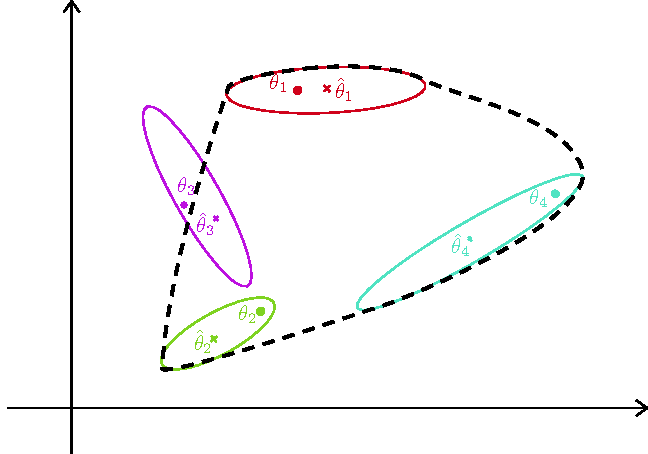
\includegraphics[width=0.5\linewidth]{images/condition_feasibility_acceptance.pdf}
	\caption{Illustrative example of condition \eqref{eq:feasibilty_condition}. The target arm is arm $3$ or $5$ and the dashed black line is the convex hull of the other confidence sets. The ellipsoids are the confidence sets $\mathcal{C}_{t,a}$ for each arm $a$. If we consider only arms $\{1,2,4,5\}$, and we use $5$ as the target arm, the condition \eqref{eq:feasibilty_condition} is satisfied as there is a $\theta$ outside the convex hull of the other confidence sets. On the other hand, if we consider arms $\{1,2,3,4\}$ and we use $3$ as the target arm, the condition is not satisfied anymore.}
\vspace{-.1in}
\end{figure}

\changebr{Let us assume that \changebrtwo{there is an arm in $a^\dagger\in A^\dagger$ which is} optimal for some contexts. More formally, there exists a subspace $V\subset \mathcal{D}$ such that:} 
\begin{equation*}    
\forall x\in V, \exists a^{\dagger}_{\star}(x)\in A^\dagger, \forall a\in \llbracket 1, K\rrbracket\setminus\{a^{\dagger}_{\star}(x)\} \qquad \langle x, \theta_{a^{\dagger}_{\star}(x)}\rangle > \left\langle x, \theta_{a}\right\rangle.
\end{equation*}
\changebr{We also assume that} the distribution of the contexts is such that, for all $t$, $\mu := \mathbb{P}\left(x_{t}\in V\right) >0$.
Then\changebr{,} the regret is lower-bounded in expectation by:
\begin{align*}
    \mathbb{E}(R_{T}) &= \mathbb{E}\left(\sum_{t=1}^{T} \mathds{1}_{\{x_{t}\in V\}}\big( \left\langle x_{t}, \theta_{a^{\dagger}_{\star}(x_{t})} - \theta_{a_{t}}\right\rangle\big)\right) \geq \mu m(T) \min_{x\in V} \max_{a\neq a^{\dagger}_\star(x)} \langle \theta_{a^{\dagger}_{\star}(x)} - \theta_{a}, x\rangle
\end{align*}
where $m(T)$ is the expected number of times $t\leq T$ such that condition \eqref{eq:feasibilty_condition} is not met. \changebr{\linucb guarantees that}  $\mathbb{E}(R_{T}) \leq \mathcal{O}(\sqrt{T})$ for every $T$. Hence, $m(T) \leq \mathcal{O}\left(\frac{\sqrt{T}}{\mu\min_{x\in V}\max_{a\neq a^{\dagger}_\star(x)} \langle \theta_{a^{\dagger}_{\star}(x)} - \theta_{a}, x\rangle}\right)$. This means that, in an unattacked problem, condition \eqref{eq:feasibilty_condition} is met $T - \mathcal{O}(\sqrt{T})$ times. On the other hand, when the algorithm is attacked the regret of \linucb is not sub-linear as the confidence bound for the target arm is not valid anymore. Hence we cannot provide the same type of guarantees for the attacked problem.


